%https://docs.arduino.cc/tutorials/nicla-vision/proximity

\section{Proximity Detection with Arduino Nicla Vision}

Learn how to use the proximity sensor to vary the speed of the LED's blink.

\subsection{Overview}

In this tutorial you will use the Nicla Vision to detect proximity, thanks to the Time of Flight (ToF) sensor VL53L1X.

This tutorial goes through how to create a sketch that will blink the built-in RGB LED and control the speed of its blink with the proximity values. It can be useful for future projects where there is a need to control the camera only when something is detected in front of the sensor.

The Arduino sketch shown is available inside the  library \FILE{Arduino\_Pro\_Tutorials}by going to Examples > Nicla Vision > Proximity\_Blink

\subsection{Goals}

The goals of this project are:

\begin{itemize}
  \item Set up the needed libraries
  \item Learn how to interact with the proximity readings
  \item Change the RGB values of the LED
\end{itemize}

Required Hardware and Software

\begin{itemize}
  \item Nicla Vision board
  \item VL53L1X library (Available in the Library Manager)
\end{itemize}

\subsection{Instructions}

Time of Flight Sensor

\begin{figure}
    \centering
    
    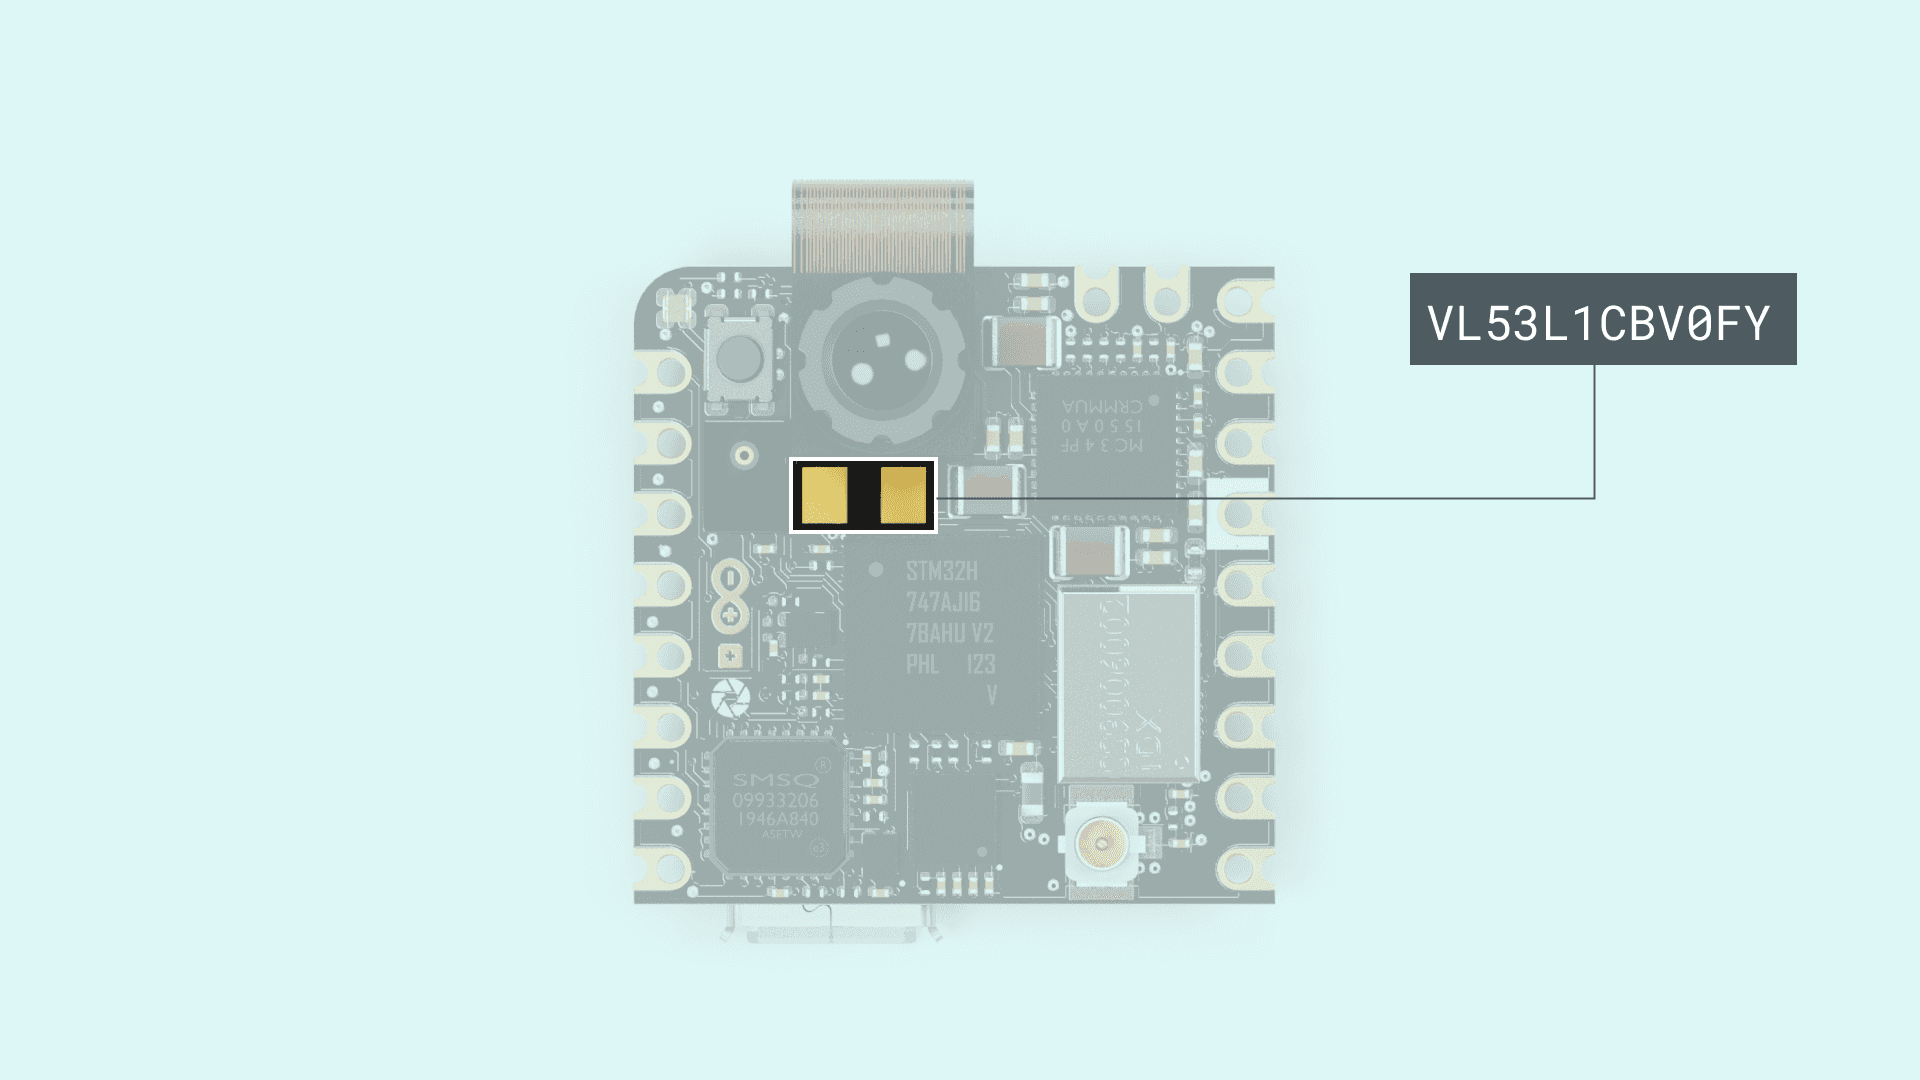
\includegraphics[width=0.5\textwidth]{IMU/nicla-vision-tof}
    
    \caption{Arduino Nicla Vision - Time of Flight sensor}\label{Proximity}
\end{figure}


To make sure that the sketch works properly, the latest versions of the Arduino mbed Core and the VL53L1X library needs to be installed. Both can be found inside the Arduino IDE.

\begin{itemize}
  \item The Arduino mbed Core can be found in the boards manager \ldots
  \item The VL53L1X library can be found in the Library manager,
\end{itemize}

If you are using version 1.6.2 or later of the Arduino software (IDE), you can use the Library Manager to install the VL53L1X library:

\begin{itemize}
  \item In the Arduino IDE, open the "Sketch" menu, select ``Include Library'', then ``Manage Libraries\ldots ''.
  \item Search for ``VL53L1X''.
  \item Click the VL53L1X entry in the list, authored by Pololu.
  \item Click ``Install''. More detailed instructions on how to install a library can be found here.
\end{itemize}


\subsubsection{Include the Needed Libraries and Objects Declaration}


First of all declare the sensor's class so you can access it later on in your sketch. We use variables to control the time elements in the sketch. This will make sure that the readings stay accurate over time.

\subsubsection{Initialize the Proximity Sensor and the LED}

Inside the setup you need to initialize and configure the proximity sensor. Also the RGB LED needs to be set as an output to make it light up and enable us to change its behavior.

\bigskip

\textbf{Note:} The LEDs are accessed in the same way as on the Portenta H7: LEDR, LEDG and LEDB

\bigskip

\textbf{Note:} Make sure you initialize Wire1, set the clock speed to 400kHz and set the bus pointer to Wire1, it won't work if you don't add these setting
    
\bigskip

\subsubsection{Control the Speed of the Blink}

The sketch is going to get the reading on every loop, store it and then the state of the LED will change, until the time is up and another proximity reading is taken.

\subsubsection{Complete Sketch}


\begin{code}
    {\scriptsize
        \lstinputlisting[language=C++]{../../Code/Arduino/Proximity/Proximity.ino}
    }
    \caption{Proximity-Sketch}\label{ProximitySketch}
\end{code}

\subsubsection{API}


\begin{table}
  \begin{tabular}{l|l|l}
    Command &	Details &	type \\ \hline
    \PYTHON{setAddress(newAddress)} &	Change the I2C sensor's address (Mandatory to set it to Wire1)	& \PYTHON{void} \\
    \PYTHON{getAddress()} & Get the Sensor's I2C address	 & \PYTHON{uint8\_t} \\
    \PYTHON{init()} &	Configures the sensor and needed data. Like the usual begin()	& \PYTHON{void}  \\
    \PYTHON{setDistanceMode(mode)} & Set the distance mode (check the datasheet). Available modes VL53L1X::Short, VL53L1X::Medium, VL53L1X::Long, VL53L1X::Unknown & \PYTHON{void} \\
    \PYTHON{getDistanceMode()} &  	Returns the mode that has been set. Available modes VL53L1X::Short, VL53L1X::Medium, VL53L1X::Long, VL53L1X::Unknown	& \PYTHON{enum DistanceMode}  \\
    \PYTHON{setMeasurementTimingBudget(uSeconds)} &	Set the time to get the measure, greater the value, better precision. In micro seconds. &	\PYTHON{void} \\
    \PYTHON{getMeasurementTimingBudget()} &	Get the measure timing value in micro seconds. &\PYTHON{uint32\_t} \\
    \PYTHON{startContinuous()} & Start the non stop readings, set the period inside the parameter, after that time you will get the reading. &	\PYTHON{void} \\
    \PYTHON{stopContinuous()} &	Stop the non stop measurements.	& \PYTHON{void}\\
    \PYTHON{read()}	& Get the last reading from the continuous mode. &	\PYTHON{void} \\
    \PYTHON{readSingle()}	& Trigger one reading and get its result.& 	\PYTHON{uint16\_t} \\
    \PYTHON{dataReady()}	& Returns if the sensor has new data available.	& \PYTHON{bool} \\
    \PYTHON{setTimeout(mSeconds)} &	Configure the milliseconds the sensor will wait in case it is not getting the proper reading to abort, and continue with a new one, 0 disables it.	& \PYTHON{void} \\
    \PYTHON{getTimeout()} & Get the configured timeout value. & \PYTHON{uint16\_t} \\
    \PYTHON{timeoutOccurred()}	& Returns true whenever the sensor had a timeout. & \PYTHON{bool} \\
  \end{tabular}
\end{table}

\subsection{Conclusion}

In this tutorial we went through how to get readings from the ToF sensor. And how use these readings to change how the built-in LED behaves. At the end of the tutorial you can also find a reference list for the ToF library.
